\documentclass[a4paper,11pt]{article}
\usepackage{pgfplots}
\usepackage{filecontents}
\begin{filecontents*}{readme.md}
Renders a background colour in a 
pgfplot.
\end{filecontents*}
\pgfplotsset{width=7cm,compat=1.5}
\usetikzlibrary{backgrounds}
% background color definition from pgfmanual-en-macros.tex
\definecolor{graphicbackground}{rgb}{0.96,0.96,0.8}
% key to change color
\pgfkeys{/tikz/.cd,
  background color/.initial=graphicbackground,
  background color/.get=\backcol,
  background color/.store in=\backcol,
}
\tikzset{background rectangle/.style={
    fill=\backcol,
  },
  use background/.style={    
    show background rectangle
  }
}

\begin{document}
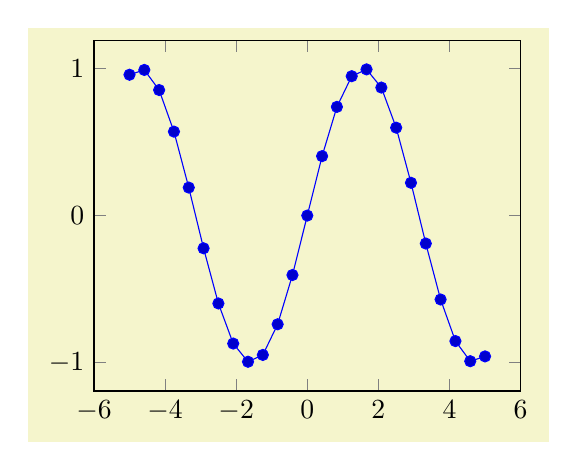
\begin{tikzpicture}[use background]
\begin{axis}
\addplot {sin(deg(x))};
\end{axis}
\end{tikzpicture}
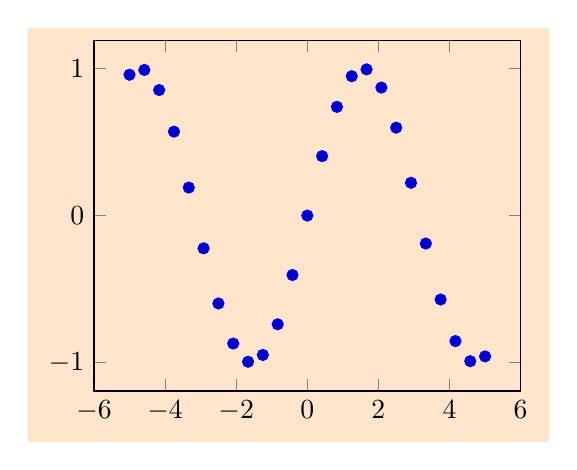
\begin{tikzpicture}[background color=orange!20,use background]
\begin{axis}
\addplot+[only marks] {sin(deg(x))};
\end{axis}
\end{tikzpicture}
read this

http://tex.stackexchange.com/questions/95687/what-are-coding-conventions-in-latex/95723#95723

I am familiar with two general approaches to creating unreadable and unmanageable software.

The first one is to take logically unrelated operations and combine them into one giant blob via shared/global variables and god objects/methods. This is what commonly known as spaghetti code.

The second one it to take every piece of functionality and shatter it into tiny pieces, so no unit of code represents anything anymore. This can be done with endless callbacks or layers of abstraction, and it can be made worse by complex frameworks with a lot of "magic" taking place or a lot of boilerplate being required. I don't know any common name for this, but let's call it mush coding.

It looks like the post describes how to convert moderately readable spaghetti code into unreadable mush code. (I would claim that a person not familiar with JQuery could easily understand the initial code, while a person not keenly familiar with Backbone would be completely lost in the final version.)

If most of your methods are longer than 100 lines, something is probably wrong. If most of your methods are shorter than 3 lines, something is probably wrong as well.

romaniv on HN http://news.ycombinator.com/item?id=5128503
\end{document}